% Short Sectioned Assignment
% LaTeX Template
% Version 1.0 (5/5/12)
%
% This template has been downloaded from:
% http://www.LaTeXTemplates.com
%
% Original author:
% Frits Wenneker (http://www.howtotex.com)
%
% License:
% CC BY-NC-SA 3.0 (http://creativecommons.org/licenses/by-nc-sa/3.0/)
%
%%%%%%%%%%%%%%%%%%%%%%%%%%%%%%%%%%%%%%%%%

%----------------------------------------------------------------------------------------
%	PACKAGES AND OTHER DOCUMENT CONFIGURATIONS
%----------------------------------------------------------------------------------------

\documentclass[paper=a4, fontsize=11pt]{scrartcl} % A4 paper and 11pt font size

\usepackage[T1]{fontenc} % Use 8-bit encoding that has 256 glyphs
\usepackage[english]{babel} % English language/hyphenation
\usepackage{amsmath,amsfonts,amsthm} % Math packages


\usepackage{graphicx}
\usepackage{subfig}
\usepackage{amssymb}
\usepackage{hyperref}
\usepackage{float}

\usepackage{multicol}
\usepackage{mdwlist}
\usepackage{fancyhdr} % Custom headers and footers
\pagestyle{fancyplain} % Makes all pages in the document conform to the custom headers and footers
\fancyhead{} % No page header - if you want one, create it in the same way as the footers below
\fancyfoot[L]{} % Empty left footer
\fancyfoot[C]{} % Empty center footer
\fancyfoot[R]{\thepage} % Page numbering for right footer
\renewcommand{\headrulewidth}{0pt} % Remove header underlines
\renewcommand{\footrulewidth}{0pt} % Remove footer underlines
\setlength{\headheight}{6pt} % Customize the height of the header

\numberwithin{equation}{section} % Number equations within sections (i.e. 1.1, 1.2, 2.1, 2.2 instead of 1, 2, 3, 4)
\numberwithin{figure}{section} % Number figures within sections (i.e. 1.1, 1.2, 2.1, 2.2 instead of 1, 2, 3, 4)
\numberwithin{table}{section} % Number tables within sections (i.e. 1.1, 1.2, 2.1, 2.2 instead of 1, 2, 3, 4)

\setlength\parindent{0pt} % Removes all indentation from paragraphs - comment this line for an assignment with lots of text

%----------------------------------------------------------------------------------------
%	TITLE SECTION
%----------------------------------------------------------------------------------------

\newcommand{\horrule}[1]{\rule{\linewidth}{#1}} % Create horizontal rule command with 1 argument of height

\title{	
\normalfont \normalsize 
\textsc{UC Berkeley, Computer Science} \\ [25pt] % Your university, school and/or department name(s)
\horrule{0.5pt} \\[0.4cm] % Thin top horizontal rule
\huge Gender Classification of Handwritten Text \\ % The assignment title
\horrule{2pt} \\[0.5cm] % Thick bottom horizontal rule
}

\author{Peter Cheng, Jeff Tsui, Alice Wang} % Your name

\date{\normalsize\today} % Today's date or a custom date

\begin{document}

\maketitle % Print the title

\section{Introduction}
For our project we designed and tested an off-line classifier for
gender prediction using handwritten text. The inspiration for this
project came from a Kaggle machine learning competition
\cite{kaggle}. Kaggle provides sample training data, in the form of
high-resolution (300 dpi) jpg images. Each image corresponds to a
writing sample, and there are 4 writing samples for each of 475
writers. The 4 samples correspond to:

\begin{enumerate}
\item Arabic text, different text for each writer
\item Arabic text, same text for each writer
\item English text, different text for each writer
\item English text, same text for each writer
\end{enumerate}

Section \ref{sec:background} provides some details that lead to
preprocessing and feature extraction. Section \ref{sec:pands} details
the preprocessing tasks we performed on the Kaggle jpg images
provided. Section \ref{sec:feature} describes in detail the
methodology behind feature extraction of the processed images. Section
\ref{sec:results} demonstrates the performance of our extracted
features using various canonical classifiers.

\section{Background}
\label{sec:background}
For this particular contest, Kaggle provides 7067 extracted features
for each of the 1128 writing samples across 282 writers. In an attempt
to simplify the problem, we opted to consider only the fourth sample
for each writer, which is the same English text written by each
writer. Since the data supplied is for a competition, the test data
did not have gender labels. We thus limited our dataset to the labeled
training data, where label = 1 for male and label = 0 for female writers. Of
these 282 writing samples, we reserved 25\% to be our testing set.

An example of a document image from our dataset is shown in Figure
\ref{fig:docImage}. As evident in the image, the handwritten text is a
color image, and the contour of each line is unconstrained. Upon
relevant literature review, we discovered that properly handling such
unconstrained data, and gathering useful features from them is a very
interesting and active research area. We thus focused our project on
performing our own text segmentation and feature extraction.


\begin{figure}
  \centering \fbox{\includegraphics[width=4in,
    height=5in]{docimage.jpg}}
  \caption{A sample input document image}
  \label{fig:docImage}
\end{figure}

We initially attempted to perform Optical Character Recognition on
each image, in an attempt to link handwritten text across images,
though we obtained poor results, and introduced more error and
uncertainty than needed. Instead, we independently performed a number
of preprocessing, segmentation, and feature detection steps as will be
described in the following sections. Throughout this paper, we will
refer to document images as images containing a single document, while
word images and line images correspond to images containing a single
word or line respectively.

\section{Preprocessing and Segmentation}
\label{sec:pands}
Typically, when performing handwriting classification and feature
extraction, binary images with a number of constraints are
assumed. Typical constraints seen in previous works include having
images in black and white text, all equally scaled among different
writers, and lines written at consistent angles
\cite{Preprocessing}. Furthermore, many feature extraction approaches
are tuned to work on images of individual characters, words, or lines,
instead of an entire document altogether. As a result, prior to
feature extraction, we perform a series of preprocessing steps to
normalize each document image, followed by segmentation procedures to
isolate individual lines and words.

\subsection{Preprocessing}
The first step in preprocessing is to translate each input color image
into a binary black and white image. To accomplish this, an intensity
threshold is calculated, such that pixels with intensity above that
value are set to 1, while the rest are set to 0. This intensity
threshold is calculated using Matlab's ``graythresh'' function, which
performs Otsu's method for binary thresholding
\cite{ThresholdSelection}. Following this binarization, we then trim
off the margins of each image, as writing samples are centered around
different locations on the page. This is accomplished by retaining the
image within the minimum axis-aligned bounding box containing all text
in the image.

\subsection{Segmentation}
While features that are calculated on handwriting samples could
theoretically be extracted from entire document images all at once,
many of the features we use are specific to words or lines, so it
makes sense to first break down the input space into line images and
word images, so as to potentially reduce error when extracting these
features.

\subsubsection{Line Segmentation}

\begin{figure}
  \centering 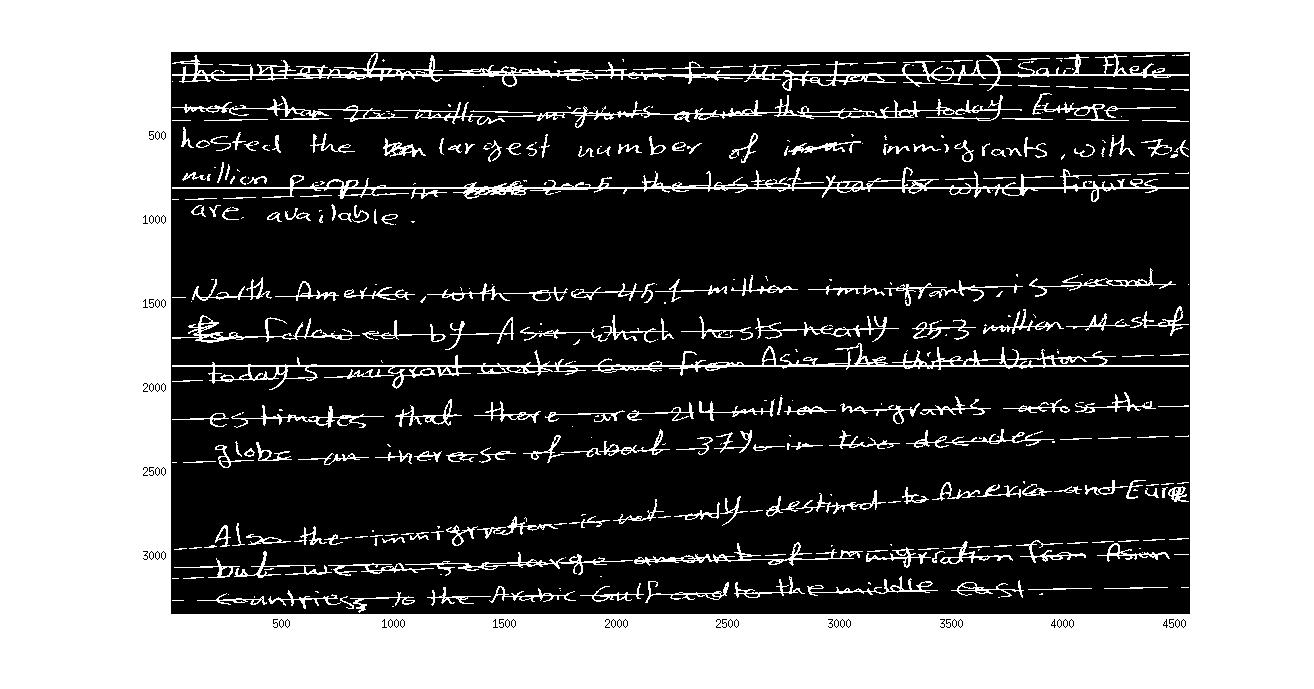
\includegraphics[width=4in,
  height=4in]{linesdetected.jpg}
  \caption{Line segments detected on a document image roughly
    correspond to lines of text}
  \label{fig:houghLineDetect}
\end{figure}

To perform line segmentation, the Hough-transform-based algorithm
proposed by Louloudis, G., et al, \cite{BlockBased} is loosely
followed. First, we use Matlab's probabilistic Hough line segment
detector (HoughlinesP) implementation to detect lines on the document
images, preprocessed after the previous section. We restricted Hough
peak detection to only occur in the angle domain such that detected
lines deviate at most 5 degrees from horizontal. We binned angles at a
resolution of 1 degree, and the rho parameter at a resolution of 1
pixel. Since the parameters for minimum line length and maximum gap
within a line are more important, they are set to be 75\% of the
image's width and 10\% of the image's width. An example of such
detected lines is shown in Figure \ref{fig:houghLineDetect}. Each
detected line is then ``drawn'' onto the word image, such that pixel
values corresponding to the line are set to 1. Next, connected
components are detected on the resulting image. The effect of drawing
each detected line upon the image is such that each character and word
in a line of text should now all be in one contiguous connected
component held together by the lines drawn over them. Connected
components with fewer than 10000 pixels were filtered as they often
correspond to punctuation or characters that were not properly
grouped. Connected components with a width less than 8 times their
height are also discarded, since they generally correspond to cases
where multiple lines of text are detected together. Each connected
component is now output at as a separate line of text.

In some cases, our line segmentation technique is unable to correctly
separate adjacent lines. An example of this is seen in Figure
\ref{fig:linefail}, where the two lines present are both angled and
very close together.

\begin{figure}
  \centering 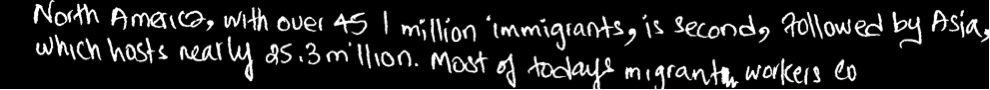
\includegraphics{linefail.png}
  \caption{In this case, line segmentation failed to perform properly
    because two lines were very close together and a single detected
    line segment spanned both lines.}
  \label{fig:linefail}
\end{figure}

\subsubsection{Word Segmentation}
For word segmentation, we use a method similar to the line
segmentation method described in the previous section. Beginning with
line images, shorter lines are detected and drawn, such that each word
is its own connected component. We use the same angle and offset
thresholds and resolutions as before, but set the minimum line length
to be 2\% of the line image's width, and the maximum gap in a line is
1.5\% of the line image's width. After filtering out connected
components with fewer than 500 pixels, we can then extract word images
via the connected components. As seen in Figure \ref{fig:wordfail},
this works well for a high percentage of words but does not in certain
cases. The writer used cursive writing with little spacing between
consecutive words, which resulted in the three words ``there'',
``are'', and ``21'' being are segmented as one word.


It is useful to have words that are rotated such that their baseline
is horizontal during feature extraction. Caesar, T., et al
\cite{Preprocessing} cite a number of approaches to accomplish this,
but we use a fairly simple approach. For each word, we compute its
(rotated) bounding box, and rotate the image such that the bounding
box is axis-aligned.

\begin{figure}
  \centering 
\includegraphics{wordfail.png}
  \caption{A case where word segmentation does not perform properly,
    as adjacent words are connected or close together.}
  \label{fig:wordfail}
\end{figure}


\section{Feature Extraction}
\label{sec:feature}
In this section, we describe the features recovered from line images
and word images, after preprocessing and segmentation, as described in
the previous two sections. A listing of each feature is shown in
Figure \ref{fig:featureList}.

\begin{figure}
  \begin{multicols}{3}
    \begin{enumerate*}
    \item Upper baseline to top line distance
    \item Lower baseline to upper baseline distance
    \item Bottom line to lower baseline distance
    \item 1 / 2
    \item 1 / 3
    \item 2 / 3
    \item Median of the gap lengths
    \item 2 / 7
    \item Average slant angle
    \item Std dev of slant angles
    \item Line angle
    \item Slant of lower contour
    \item Mean squared error of lower contour
    \item Freq of local max for lower contour
    \item Freq of local min for lower contour
    \item Avg left slope of local max for lower contour
    \item Avg right slope of local max for lower contour
    \item Avg left slope of local min for lower contour
    \item Avg right slope of local min for lower contour
    \item 12 for upper contour
    \item 13 for upper contour
    \item 14 for upper contour
    \item 15 for upper contour
    \item 16 for upper contour
    \item 17 for upper contour
    \item 18 for upper contour
    \item 19 for upper contour
    \item Avg width of connected components
    \item Avg height of connected components
    \item Std dev of width of CCs
    \item Std dev of height of CCs
    \item Avg dist between adjacent CCs
    \item Std dev of dist between adjacent CCs
    \item Avg area of enclosed regions
    \item Avg length of major axis of ERs
    \item Avg length of minor axis of ERs
    \item Avg orientation of ERs
    \item Avg eccentricity of ERs
    \item Avg equiv diameter squared of ERs
    \item Avg extent of ERs
    \item Avg perimeter of ERs
    \item Avg form factor of ERs
    \item Avg roundness of ERs
    \item Std dev of 34
    \item Std dev of 35
    \item Std dev of 36
    \item Std dev of 37
    \item Std dev of 38
    \item Std dev of 39
    \item Std dev of 40
    \item Std dev of 41
    \item Std dev of 42
    \item std dev of 43
    \item Fractal dimension slope 1
    \item Fractal dimension slope 2
    \item Fractal dimension slope 3
    \end{enumerate*}
  \end{multicols}
  \caption{The features we extracted from each input document image}
  \label{fig:featureList}
\end{figure}

\subsection{Word Features}
The first group of features are generated based on word images,
referencing the work of Marti, U.-V., et al \cite{WriterID} where a
feature vector is extracted from each word. These feature vectors are
averaged by line to combine them with line-specific feature
vectors. The word features are comprised of the width, slant, and
height of the three main writing zones, described below.

\subsubsection{Word Height}
The three writing zones are separated by the upper and lower
baselines. The upper and lower baselines are defined via a histogram of the number of black pixels in every line; 15\% of black pixels exist above the upper baseline and 90\% of black pixels
exist above the lower baseline. An example is shown in Figure
\ref{fig:wordheight}. The baselines are used to extract features 1
through 6, which include the distance between the upper and lower baselines and the top and bottom lines, where the top line is the first row of the image and the bottom line is the bottom row. These features encode the height of the handwriting. The ratios of 1, 2, and 3 are taken to adjust for the variation in word size between writing samples.

\begin{figure}
  \centering 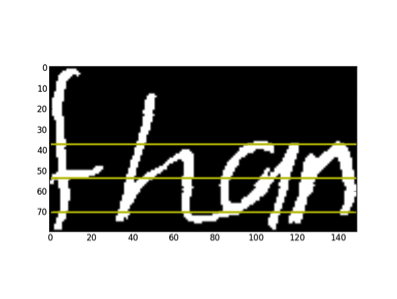
\includegraphics[width=2in]{wordheight.png}
  \caption{The upper and lower baselines are shown in this
    example. The middle baseline is also shown and lies halfway between the upper and lower
    baselines.}
  \label{fig:wordheight}
\end{figure}

\subsubsection{Word Width}
The row with the most black and white transitions defines the width of
words. To represent the width of the writing, the number of white gaps
between every group of black-white-black pixels is calculated and the
median of these values is taken. Again, the ratio is taken with feature 2,
the vertical height of the middle portion of the writing to account
for the word size variation between writers. An example of this is
shown in Figure \ref{fig:wordwidth}

\begin{figure}
  \centering 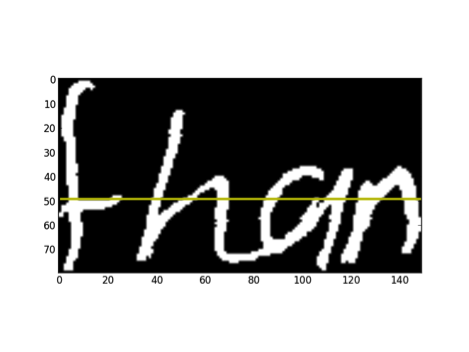
\includegraphics[width=2in]{wordwidth.png}
  \caption{The line drawn in this image contains the most black/white
    transitions}
  \label{fig:wordwidth}
\end{figure}

\subsubsection{Word Slant}
We created a histogram of angles for each word in order to calculate
the slant of the handwriting. First we converted the image to an outline such
that only the perimeter pixels at the edge of each word remain. For
each black pixel in the middle row of the middle baseline (halfway between the
upper and lower baselines), we calculate the angle from the pixel to
a connected pixel intersecting with the upper and lower baselines. To
encode the slant for the word, we compute the average of all these angles and the standard deviation. An example of this is shown in Figure
\ref{fig:wordslant}

\begin{figure}
  \centering 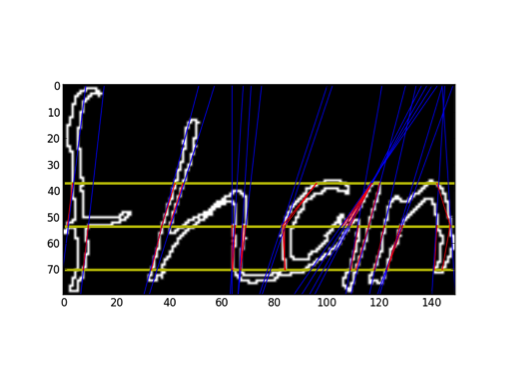
\includegraphics{wordslant.png}
  \caption{The slant of various parts of letters, as detected via
    adjacent pixels}
  \label{fig:wordslant}
\end{figure}


\subsection{Line Features}
The next group of features we generated were extracted from line
images. This includes the angle of each line, the characteristics of
its contour, various calculations performed on connected components
and enclosed regions, as well as fractal dimension. We referenced work
from Bouletreau, V., et al \cite{SyntheticParameters}, Hertel, C. and
Bunke, H., \cite{NovelFeatures}, and Vincent,
N. \cite{FractalDimensions} to create these features.

\subsubsection{Line Angle}
The first feature comes from the angle of the line. This is simply the
angles of the lines detected in Section \ref{sec:pands} when
performing line segmentation. If multiple line segments were detected
for a single line, the average of their angles is used. For subsequent
features, we use the rotated line so that writing is parallel with the
x-axis.

\subsubsection{Contour}
The upper and lower contours of a line are the sequence of uppermost
and lowermost pixels in each column of a line image. Gaps in which a column
of the image has no black pixels are removed. The characteristic
contours are generated by shifting y-coordinates of consecutive
points such that they are at most 1 pixel apart on the y-axis. This eliminates
discontinuities in the contours. Several
features are extracted from the characteristic lower and upper
contours, such as 1) the slope of the least squared regression line 2)
the mean squared error for the line 3) the frequency of local minima
and maxima, found by dividing the number of local extrema by the
length of the contour, 4) the local extrema, determined by comparing
the the neighboring three points on either side. The average slopes of
the left three points and the right three points for each local maxima
are computed, as well. Figure \ref{fig:contourimage} demonstrates an
example of an extracted contour.

\begin{figure}
  \centering 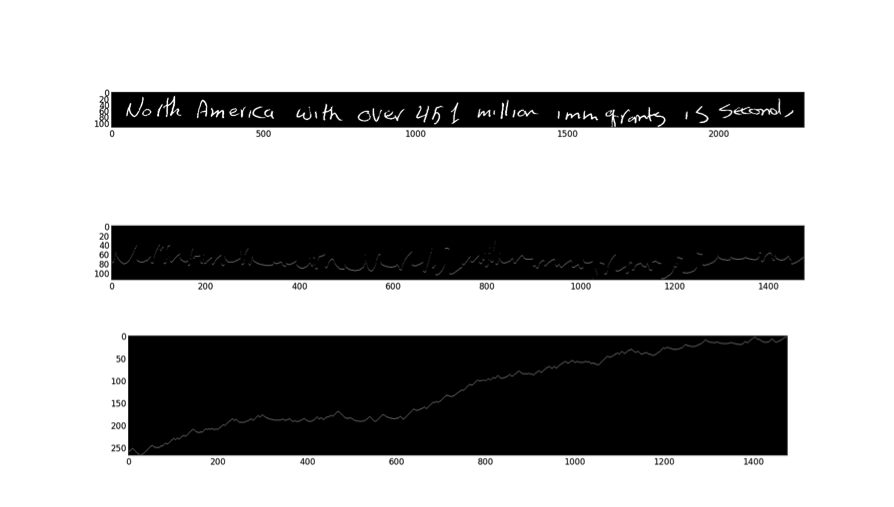
\includegraphics{contourimage.png}
  \caption{From top to bottom: the rotated line image, the lower
    contour of the line, and the lower characteristic contour.}
  \label{fig:contourimage}
\end{figure}

\subsubsection{Connected Components and Enclosed Regions}
The next two sets of features correspond to characteristics of
connected components and enclosed regions within a line of
text. Connected components will generally be larger for writers whose
handwriting is larger. Writers whose letters overwrite in handwriting
will often have very wide connected components relative to their
heights. The spacing between connected components also provides
additional information about character spacing as well. Enclosed
regions, on the other hand are the opposite of connected
components. In a line of handwriting, they correspond to areas within
loops and other enclosed areas. The roundness or eccentricity of each
enclosed region can reveal information about how slanted a text sample
is as well as the curvature of handwriting. Perimeter size contains
the size of loops in text, and numerous other calculations provide
similar characterizations of text. The features derived from connected
components and enclosed regions correspond to features 28-53 from the
table in Figure \ref{fig:featureList}.

\subsubsection{Fractal Dimensions}
Fractal dimensions encode the degree of irregularity and fragmentation
of the handwriting, from which our final three features are
derived\cite{FractalDimensions}. At a high level, they measure the space filling capacity of an image and is measured by a dilation operation on each line image. Given X as the
contour of the handwriting sample, its fractal behavior is generated
via the evolution of the areas of successive dilation sets of boxes on
its contour. Xn is the set of boxes used in the dilation for n number of boxes where each box has area A(Xn). In Figure \ref{fig:fractaldimension}, the evolution graph plotting log(n) on the x axis and log[A(Xn)] - log(n) on the y axis is shown.

Using the Minkowski-Bouligand dimension, the fractal behavior of the X
set is expressed by the linear relationship between log[A(Xn)] and
log(n) \cite{SyntheticParameters}. In plotting the x's and y's, the
fractal features are the slopes of the three-part linear regression
line that fits all possible points on the x-axis and and minimizes the
mean squared error between the original points of the graph and the
line segments\cite{GeometricalFeatures}.  The three regressions
correspond to three zones of the image: zone 0 characterizes the line
thickness, which is omitted since it varies based on resolution and
image quality; zone 1 characterizes the writing shape; and zone 2
matches the dilations from which the writing is hidden. An example
plot of 3 detected lines correspond to the 3 fractal dimension
features is shown in Figure \ref{fig:fractaldimension}

\begin{figure}
  \centering 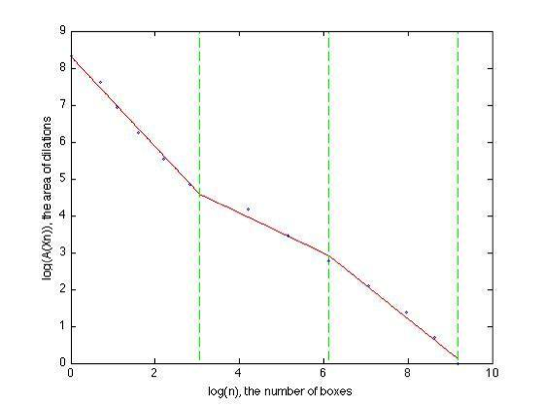
\includegraphics{fractaldimension.png}
  \caption{The slopes of the 3 straight lines that produce the best
    least squares fit constitute 3 features.}
  \label{fig:fractaldimension}
\end{figure}

\section{Results}
\label{sec:results}
In this section, we apply 4 classification techniques to 4 different
feature sets, and compare their results. Because our features are
independently acquired on a per-line basis, and the end goal is to
classify each document, we decided upon three ways to aggregate our
features and determine their performance. The first is simply to
classify each line separately, and consider our accuracy to be the
percentage of lines accurately classified. The second method is to
average the feature vectors for all lines within a document, and end
with an ``average'' line feature vector for each document. The third
method is to classify each line separately, but classify each document
based on the majority vote of its line classifications. As a
benchmark, we also acquired Kaggle's 7067-length feature vectors for
each document. Because the per-line classification method works with a
feature vector for each line, it has roughly 10x amount training and
test samples, which impacts the parameters chosen for classification,
as described later in this section. Each of these 4 feature sets was
run through the following classification techniques: linear SVM, SVM
with an RBF kernel, random forest, and k nearest neighbors. Accuracies
of each can be seen in Figure \ref{fig:resultsTable}.

\begin{figure}
  \begin{center}
    \begin{tabular} { | l | c | c | c | c | }
      \hline
      & SVM-Linear & SVM-RBF & Random Forest & kNN \\ \hline
      Kaggle Features (per document) & 75.2\% & 74.8\% & 73.8\% & 70.2\% \\ \hline
      Our Features-per line & 65.5\% & 69.4\% & 66.1\% & 57.9\% \\ \hline
      Our Features-averaged & 75.0\% & 82.4\% & 71.0\% & 73.5\% \\ \hline
      Our Features-voting & 65.5\% & 70.6\% & 69.1\% & 64.7\% \\ \hline
    \end{tabular}
  \end{center}
  \caption{Accuracy of each classification method on each feature set}
  \label{fig:resultsTable}
\end{figure}

For SVMs, we found that tweaking the C (cost) value had a strong effect on classification
accuracy. Upon cross-validating across multiple values, we ended with
a C value of 10 for the per-document feature sets, while a C value of
1 performed better for the per-line feature set. The RBF SVM also has
a $\sigma$ parameter, which strongly affects accuracy as well; we
performed cross-validation to obtain $\sigma$ of 6 and 10 for the line
and document feature sets respectively. The RBF SVM performed better
than the linear one, and in fact better than all other
classifiers. Our averaged feature vector also greatly outperformed the
other feature sets here, including Kaggle's set.

With the random forest method, we found no improvements in out-of-bag
error past 100 trees, for each feature set. The minimum leaf size
seemed to impact overfitting, and cross-validation resulted in a
minimum leaf size of 50 for line features, and 10 for document
features. Plots of the out-of-bag errors versus number of trees for
each feature set is shown in Figure \ref{fig:oob}, and their
asymptotic minimum values match the accuracies obtained.

For K nearest neighbors, we simply used euclidean distance and
cross-validated on values of k. The best values were 46, 18, 4, and 7,
for the Kaggle, per-line, averaged, and voting datasets
respectively. These numbers were not very sensitive however, in that
changing K generally had minimal effect on accuracy. Here, the
averaged dataset actually outperforms Kaggle's feature set again.

\begin{figure}
  \centering
  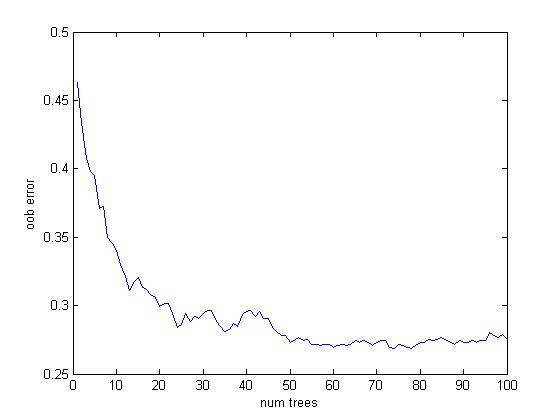
\includegraphics[width=1.4in,height=1.4in]{randforestKaggle_oob.jpg}
  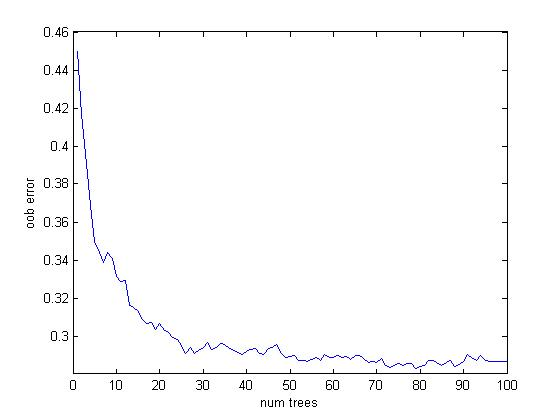
\includegraphics[width=1.4in,height=1.4in]{randforestOurs_oob.jpg}
  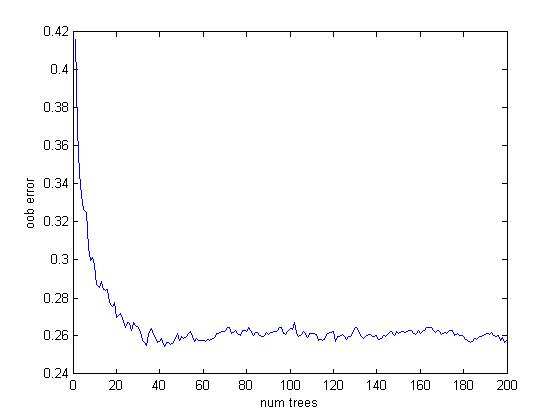
\includegraphics[width=1.4in,height=1.4in]{randforestAvg_oob.jpg}
  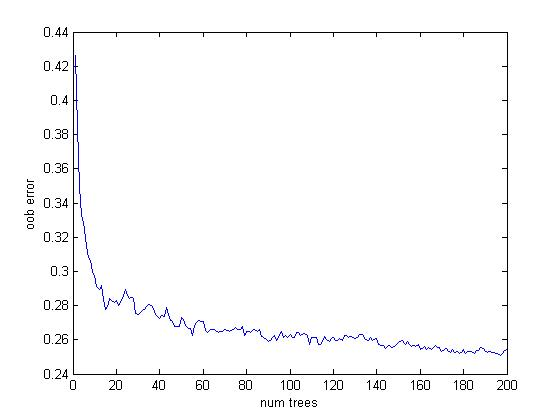
\includegraphics[width=1.4in,height=1.4in]{randforestVote_oob.jpg}
  \caption{Out of bag error plots for the Kaggle, per-line, averaged,
    and voting datasets from left to right.}
  \label{fig:oob}
\end{figure}

Across all classifiers, the averaging method outperformed the voting
method, followed by the per-line method. The per-line method performs
the worst, as it is the most sensitive to outliers or errors in either
segmentation or feature detection. The voting method performs better
for all classifiers though only minimally, or identically, in the
linear and rbf SVM. Plots of the majority classification votes
received from each line across each document are shown in Figure
\ref{fig:votes}. As evident, the linear SVM and rbf SVM plots have
many documents where all lines receive the same classification. This
is a positive result to see, as it implies that there is some amount
of clustering of each line's feature vector within a document.

Universally however, the averaging method is superior for our dataset
on each of our classification methods, even beating Kaggle's on two of
them. This suggests that there is likely a high amount of error and
variance in our features, as the voting method should perform
similarly to the averaging method, if provided with consistent line
vectors. Averaging likely improves accuracy by working with an
averaged feature vector, which is less prone to error.

\begin{figure}
  \centering
  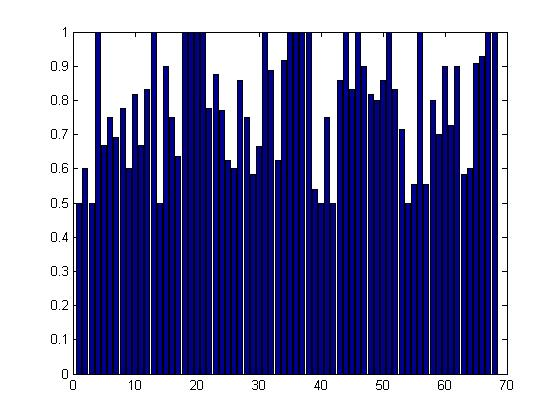
\includegraphics[width=1.4in,height=1.4in]{linearSVMVoteDistribution.jpg}
  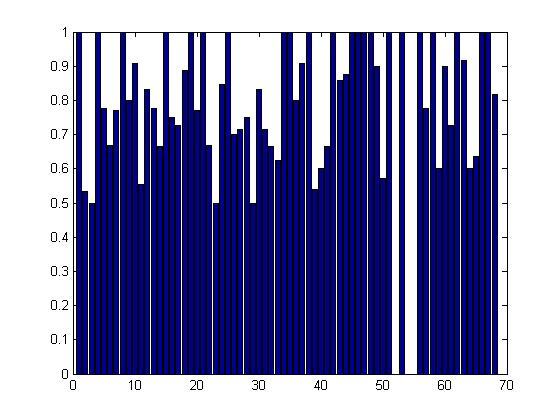
\includegraphics[width=1.4in,height=1.4in]{rbfSVMVoteDistribution.jpg}
  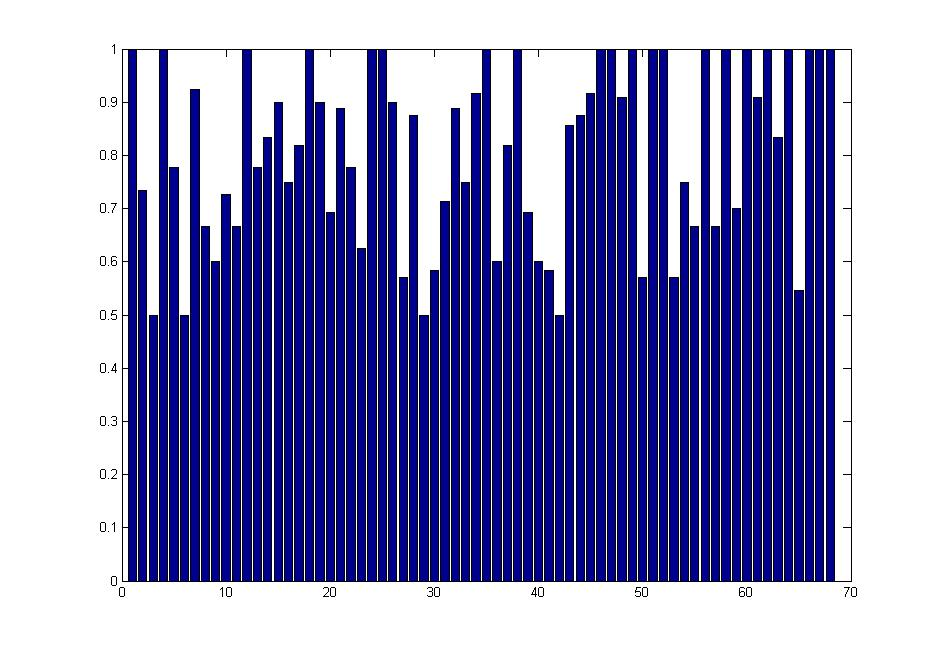
\includegraphics[width=1.4in,height=1.4in]{randForestVoteDistribution.jpg}
  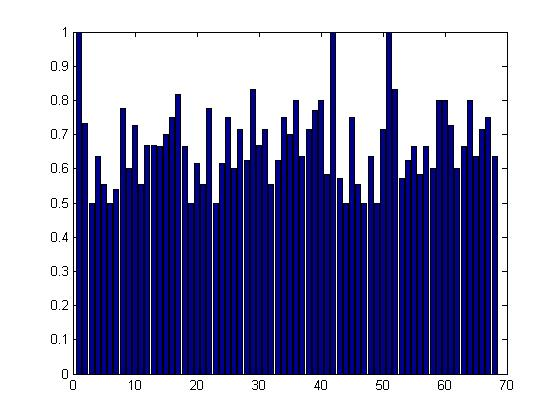
\includegraphics[width=1.4in,height=1.4in]{kNNVoteDistribution.jpg}
  \caption{Each bar represents the number of majority votes received
    on each document. Bars with values near 1 represent a high amount
    of certainty and agreement among lines in a document, while values
    near 0.5 indicate disagreement among lines. The plots are for the
    linear SVM, RBF SVM, random forest, and k nearest neighbors
    results from left to right.}
  \label{fig:votes}
\end{figure}

\section{Conclusion}
In our study of gender classification based on handwriting, we
extracted 56 features based on word and line properties and applied
several classification models. We combined these features in 3
different ways, and classified them with 4 different classifiers. To
benchmark our results, we also used the features provided in the
Kaggle competition. In general, our features resulted in slightly
higher error rates than the Kaggle feature set, though our averaging
approach resulted in comparable results. Overall, the RBF SVM
performed best, both in terms of single best accuracy, as well as
accuracy over each dataset.

While our results are somewhat lackluster for some of the
classification schemes, our focus on feature extraction was rewarded
in that some of our results are comparable to results obtained using
Kaggle's provided feature set, obtained from a number of methods coming
from recent state-of-the-art research. Furthermore, the dataset we
worked with was not very large in size, and was intended to be used in
a highly popular competition, so our results with fairly standard
classifiers are not too surprising.

Nevertheless, there are several clear ways to improve our
classification system. An improvement to our preprocessing steps that
segment documents into words and lines would result in higher accuracy
in what each feature is measuring, by reducing input error to our
feature extraction methods. Furthermore, we noticed that dividing
highly variable handwritten documents with skewed lines and different
sizes is not a trivial task. Much of our work consisted of improving
the accuracy of segmentation and reducing false positives that would
skew extracted feature vectors. This resulted in many false negatives
that greatly reduced the amount of useful input data. To further
decrease the error rate, we could continue to generate additional
features as well. The Kaggle dataset has over 7067 features, while we
achieved similar results at 56 features with rudimentary
classifiers. Finally, we extracted most of our features based on
methods developed for writer identification, since gender
classification based on handwriting is similar to writer
identification. However, it is very likely that many of the features
we implemented, designed for writer identification, may not be best
suited for the task of gender classification. For future work, 
researching for more features that detect different
properties of handwriting to better separate our data would
improve the accuracy of our classifier.



\bibliography{report} %>>>> bibliography data in report.bib
\bibliographystyle{spiebib} %>>>> makes bibtex use spiebib.bst

\end{document}